\documentclass{beamer}

% Packages likely needed by refinementtydef.sty and common usage
\usepackage{amsmath, amsfonts, mathrsfs, mathtools, stmaryrd, pifont, xcolor}
\usepackage{pict2e}
\usepackage{xspace}
\usepackage{tikz}
\usepackage{minted} 
% Note: minted requires -shell-escape flag when compiling

% Beamer theme settings
\usetheme{Madrid}
\usecolortheme{default}

% Import the custom definitions
\usepackage{hyperref, wrapfig, amsthm, pict2e, booktabs, subcaption,
  subfiles, rotating, pifont, indentfirst, amsmath, amsfonts,
  mathrsfs, adjustbox, mathtools,booktabs, microtype, ebproof,
  enumitem, multirow, multicol, setspace, xcolor, lineno, listings,
  stmaryrd, xspace, stackengine, makecell}

\usepackage{empheq}
\newcommand*\widefbox[1]{\fbox{\hspace{2em}#1\hspace{2em}}}
\usepackage[tableposition=top]{caption}
\usepackage{tikz-cd}
\usetikzlibrary{decorations.pathmorphing}
\usepackage[ruled,linesnumbered,vlined]{algorithm2e}
\newcommand\mycommfont[1]{\footnotesize\ttfamily\textcolor{DeepGreen}{#1}}
\SetCommentSty{mycommfont}
\usepackage{graphicx}
\urlstyle{same}
\usepackage{minted}
\usemintedstyle{borland}
\usepackage{tikz}
\newcounter{markeq}
\setcounter{markeq}{0}
\usepackage{spacingtricks}
\newcommand*\tstrut[1]{\vstrut{#1}}
\newcommand*\bstrut[1]{\vstrut[#1]{0pt}}
\usepackage[T1]{fontenc}
\newcommand*\mystrut[1]{\vrule width0pt height0pt depth#1\relax}
% \usepackage{bm}

\newcommand{\tyName}{\mbox{\textsf{u}\textsc{Hat}}\xspace}

% ZZ's Macros
\usepackage{spacingtricks, commands, refinementtydef}

\title{UnderType}
\author{Zhe Zhou}
\date{\today}

\begin{document}

\frame{\titlepage}

% \begin{frame}
\frametitle{Type Syntax}

The (simplified) type syntax is defined as follows:
\begin{align*}
\tau &\doteq \ort{b}{\phi} ~|~ \urt{b}{\phi} ~|~ x{:}\tau \sarr \tau ~|~ x{:}\tau \wand \tau \\
\Gamma &\doteq \emptyset ~|~ x{:}\tau ~|~ \Gamma \sep \Gamma ~|~ \Gamma, \Gamma ~|~ \textcolor{gray}{\Code{emp}}
\end{align*}

\textbf{Comparison with SL:} 

\begin{itemize}
    \item $\ort{b}{\phi}$ is similar to an atomic predicate in pure logic.
    \item $\urt{b}{\phi}$ is similar to an atomic heap predicate in heap logic (e.g., $x \mapsto 4$).
    \item $x{:}\tau \sarr \tau$ is the standard (additive, nonlinear) arrow type.
    \item $x{:}\tau \wand \tau$ is similar to a magic wand (multiplicative, linear) in separation logic.
\end{itemize}

\textbf{Note:} For now, I am not sure if I should add $\textcolor{gray}{\Code{emp}}$ to the type context syntax.

\end{frame}

\begin{frame}
    \frametitle{Type Syntax}
    
    The basic bunched type (implication) only uses connectives to separate ``heap predicates'' and ``pure logic predicates.'' The key point is that there are two unit elements (empty contexts): $\emptyset$ and $\Code{emp}$, each for a different monoid.
    \begin{align*}
    x{:}\ort{b}{\phi} &\doteq x{:}\rt{b}{\phi}, \emptyset \\
    x{:}\urt{b}{\phi} &\doteq x{:}\rt{b}{\phi} \sep \Code{emp}
    \end{align*}

    \textbf{Examples:}
    \begin{align*}
    \forall a.\exists b.\forall c &\doteq a, (b \sep (c, \emptyset)) \\
    \forall a.\exists b.\exists c &\doteq a, (b \sep c) \\
    \exists a.\forall b.\exists c &\doteq a \sep (b, (c \sep \Code{emp})) \\
    \exists a.\forall b.\forall c &\doteq a \sep (b, c)
    \end{align*}
    
    \textbf{It is too complicated; thus, we still use a more ``SL-like'' notation.} 
    
\end{frame}

\begin{frame}
    \frametitle{Type Semantics}

\begin{align*}
    \denot{ \ort{b}{\phi} } &\doteq \{ e ~|~ \forall v. \mstep{e}{v} \impl \phi[\nu\mapsto v] \} \\
    \denot{ \urt{b}{\phi} } &\doteq \{ e ~|~ \forall v. \phi[\nu\mapsto v] \impl \mstep{e}{v}  \}
\end{align*}
    
\end{frame}

\begin{frame}
    \frametitle{Stuck Term and Divergence}

\textbf{Suresh \& Ben:} It is good to compare with Ramsey's work; it is also important to distinguish between a stuck term and divergence. One terminates in a non-value normal form, while the other does not terminate.

\textbf{Suresh:} An important ``reachability'' case to consider: $\lambda x.\; 1 \oplus (2 + \true)$. This function is not well-typed in the basic type system but is still reachable in some executions. (\textcolor{red}{ZZ: I don't believe this should be a typable program to consider, especially in ML-family languages.})

\textbf{Zhe:} This seems to conflict with the idea of ``refinement type,'' where if a term $e$ has refinement type $\tau$, it means $e$ also has $\eraserf{\tau}$ in the basic type system. We also need to change the standard reduction judgment $\mstep{e}{v}$; otherwise, we cannot distinguish between a stuck term and divergence.
\begin{align*}
    &\text{standard refinement type:} \forall v. \mstep{e}{v} \impl \phi[\nu\mapsto v] \\
    &\text{stuck term:} \forall N. \mstep{e}{N} \impl \neg \Code{isValue}(N) \\
    &\text{divergence term:} \forall N. \neg \mstep{e}{N}
\end{align*}

\end{frame}

\begin{frame}
    \frametitle{Stuck Term and Divergence}

\textbf{Try:} If we do not quite follow the manner of refinement types, what can we do?

\textbf{Zhe:} $\ort{b}{\bot}$, where $b$ is an arbitrary base type, can be used to represent an ``unreachable'' term, including both stuck terms and divergence, but it cannot distinguish between them.

\textbf{Ben:} However, the basic type system can type check the divergence term. Thus, if a term can have refinement type $\ort{b}{\bot}$ and basic type $b$ in the basic type system, it is a divergence term; otherwise, it is probably a stuck term (maybe Ramsey's work can be used to prove it must get stuck).

\textbf{Suresh:} Allowing divergence and tracking it is very annoying; it needs intersection types and dynamic choice depending on the calling context. \textcolor{red}{ZZ: I agree, in some sense divergence is an effect, it is context sensitive.}

\end{frame}

\begin{frame}
    \frametitle{Stuck Term and Divergence}

\textbf{Ben:} Can we use a two-judgment design (prove $\vdash$ and disprove $\nvdash$) to type check the stuck terms?

\textbf{Zhe:} It is not quite different from Ramsey's work.

\textbf{Ben:} Should we add three or more classes of base refinement types?

\textbf{Zhe:} It is kind of ugly and complex.

\textbf{Zhe:} In some sense, our paper is about ``incorrectness reasoning,'' separation, and resource. I believe it is quite far from Ramsey's work.

\end{frame}

\begin{frame}
    \frametitle{Stuck Term and Divergence}

End here.

\end{frame}

\begin{frame}
    \frametitle{Type Semantics}

\textbf{Consider a basic type $\Int\sarr\Int$. It can have the following refinement types:}

\begin{itemize}
    \item $x{:}\ort{\Int}{\vnu > 0}\sarr\ort{\Int}{\vnu > 0}$: For all positive inputs $x$, the function diverges or returns a positive result.
    \item $x{:}\ort{\Int}{\vnu > 0}\sarr\urt{\Int}{\vnu > 0}$: coverage type (similar to $\lambda x. \Code{alloc(posGen\;())}$ in SL).
    \item $x{:}\ort{\Int}{\vnu > 0}\wand\ort{\Int}{\vnu > 0}$: fallback to the normal arrow.
    \item $x{:}\ort{\Int}{\vnu > 0}\wand\urt{\Int}{\vnu > 0}$: fallback to the normal arrow.
\end{itemize}

\textbf{Compare with SL:} $x = 3 \wand y =  5$ fallback to $x = 3 \impl y = 5$.

\textbf{Note:} in Iris style triple, them are equal to:
\begin{align*}
    &\{x > 0 \land \textcolor{red}{\Code{emp}}\} y = ... \{ y > 0 \land \Code{emp} \} 
    \\&\{x > 0 \land \textcolor{red}{\Code{emp}}\} y = ... \{ y \mapsto \Code{posGen()} \} 
\end{align*}
Overapproximation clearly requires no resource.
    
\end{frame}

\begin{frame}
    \frametitle{Type Semantics}

\textbf{Consider a basic type $\Int\sarr\Int$. It can have the following refinement types:}

\begin{itemize}
    \item $x{:}\urt{\Int}{\vnu > 0}\wand\ort{\Int}{\vnu > 0}$: there exists a input such that the return is positive or diverges.
    \item $\lambda x. x - 100$ and $\Code{fix}\;f\;x. f\;x$ has this type; $\lambda x. 0 \oplus 1$ does not have this type.
    \item $x{:}\urt{\Int}{\vnu > 0}\wand\urt{\Int}{\vnu > 0}$: incorrectness triple (be careful with variable references).
    \item $\lambda x. x - 1$ has this type.
    \item $x{:}\urt{\Int}{\vnu > 0}\sarr\ort{\Int}{\vnu > 0}$: we require that the input must be able to cover all positive integers, and the result is positive (this application will not consume resources).
    \item $x{:}\urt{\Int}{\vnu > 0}\sarr\urt{\Int}{\vnu > 0}$: it is ill-defined, 
\end{itemize}

Requiring a ``resource'' but not consuming it is a little bit weird.
    
\end{frame}

\begin{frame}
    \frametitle{Type Semantics}

\textbf{To be concrete, what is the meaning of $x{:}\urt{b}{\phi}\sarr\ort{\Int}{\vnu > 0}$?}

\begin{itemize}
    \item $\lambda x. x - 100$ has type $x{:}\urt{\Int}{\top}\wand\ort{\Int}{\vnu > 0}$; if you give me a ``coverage guarantee,'' we now comsume it and return a positive result.
    \item $\lambda x. 1$ has type $x{:}\urt{\Int}{\top}\sarr\ort{\Int}{\vnu > 0}$; if you give me a ``coverage guarantee,'' I don't consume it and still return a positive result.
\end{itemize}

$\lambda x. 1$ can also have type $x{:}\ort{\Int}{\top}\sarr\ort{\Int}{\vnu > 0}$. In the CBV incorrectness reasoning setting, we have no way to check if a parameter has a ``coverage guarantee.''
    
\end{frame}

\begin{frame}
    \frametitle{Type Semantics: affine}

\textbf{Tricky case: $x{:}\urt{b}{\vnu > 0}\sarr\urt{\Int}{\vnu > 0}$?}

\textbf{SL: $\{x \mapsto 3\} e \{y \mapsto 3\}$?}

\begin{itemize}
    \item Standard SL: before execution I have a heap with singleton address $x$, after execution I have a heap with singleton address $y$. It may because $x = y$ and I do nothing, or $x \neq y$ and I free $x$ and allocate a new address $y$.
    \item Affine SL (e.g., Iris): I allow not to describe the state of address $x$ after execution, thus the $x$ can be not freed.
\end{itemize}

If we choose the first interpretation, it is the same with $x{:}\urt{b}{\vnu > 0}\wand\urt{\Int}{\vnu > 0}$.

If we choose the second interpretation, it is similar with $x{:}\ort{b}{\vnu > 0}\sarr\urt{\Int}{\vnu > 0}$.

In our pure functional setting, the function cannot modify the argument; the state of input argument is in charge of typing rules. We choose the interpretation similar with the second.
    
\end{frame}

\begin{frame}
    \frametitle{Type Semantics}

\textbf{It seems that we always have:}

\begin{itemize}
    \item $x{:}\ort{\Int}{\phi}\sarr\tau$: the normal arrow means over parameters.
    \item $x{:}\urt{\Int}{\phi}\wand\tau$: the magic wand means under parameters.
\end{itemize}
    
\end{frame} 

\begin{frame}[fragile]
    \frametitle{Resource Semantics: an SL-style Interpretation}

    \textbf{In order to explicitly show the meaning of resource in our setting:}

\textbf{A heap-based (modal logic style) interpretation:} We assume the under-type denotation is parameterized by a heap; coverage means there exists a heap makes it holds.

\textbf{Qualifier logic:} we allow $!x$ represents the value of address $x$ store in the heap.

\textbf{Type Context:} $x{:}\urt{b}{\phi}$ means some constraint about the assignment of $x$, and also \textbf{a singleton resource (heap)}.
\begin{align*}
    x{:}\urt{b}{\phi} \doteq \exists i{:}\Code{Addr}.\exists v{:}\Code{Choice}.\exists f{:}\Code{Choice}\sarr \rt{b}{\phi}. i\mapsto v \land x = f(v)
\end{align*}
Here, $i$ is an address, $v$ is a \emph{choice} that is stored at this address, and $f$ is a \textbf{surjective} function mapping a value of type $\Code{Choice}$ to (refined) type $b$ with qualifier $\phi$. 

Note that in order to make $f$ well-defined, we require $|\Code{Choice}| \geq |t|$ for any basic type $t$ (e.g., $|\Code{Choice}| = 2^{\aleph_0}$).

\end{frame}

\begin{frame}[fragile]
    \frametitle{Resource Semantics: an SL-style Interpretation}

\textbf{Type Context:} $x{:}\urt{b}{\phi}$ means some constraint about the assignment of $x$, and also \textbf{a singleton resource (heap)}.
\begin{align*}
    x{:}\urt{b}{\phi} \doteq \exists i{:}\Code{Addr}.\exists v{:}\Code{Choice}.\exists f{:}\Code{Choice}\sarr \rt{b}{\phi}. i\mapsto v \land x = f(v)
\end{align*}

\textbf{This means:} The value of $x$ depends on a heap fragment with address $i$; when the value $v$ is stored at this address, the value of $x$ is $f(v)$, since $f$ is surjective to the codomain $\rt{b}{\phi}$, the assignment of $x$ can cover $\phi$.

\textbf{Key:} The value of $x$ is fully determined by the heap fragment and the function $f$.

\end{frame}

\begin{frame}[fragile]
    \frametitle{Resource Semantics: an SL-style Interpretation}

\textbf{A heap-based interpretation:}
\begin{align*}
    x{:}\urt{b}{\phi}, y{:}\urt{b}{\phi} 
\end{align*}
means
\begin{align*}
    \exists v_1, v_2. (i_1 \mapsto v_1 \land x = f_1(v_1)) \land (i_2 \mapsto v_2 \land y = f_2(v_2))
\end{align*}
Here, the conjunction does not guarantee the separation of $i_1$ and $i_2$; or it assumes $f_1$ and $f_2$ share the same heap address, that is,
\begin{align*}
    \exists v. i \mapsto v \land x = f_1(v) \land y = f_2(v)
\end{align*}

\textbf{Key:} According to $\exists v. x = f_1(v)$, the assignment to $x$ can still cover the codomain of $f_1$, and similarly for $y$. However, $x$ and $y$ are not independent.
\end{frame}

\begin{frame}[fragile]
    \frametitle{Resource Semantics: a Formal Definition}

\textbf{A resource-based type denotation:} The denotation of a type context is a substitution \textbf{plus a set of heap addresses (or, abstractly, resource identifiers)}.
\begin{align*}
    \denot{\emptyset} &\doteq (\emptyset, \sigma_{\Code{id}}) \\
    \denot{x{:}\ort{b}{\phi}} &\doteq \{ (I, [x\mapsto v]) ~|~ v \in \denot{\ort{b}{\phi}} \} \\
    \denot{x{:}\urt{b}{\phi}} &\doteq \{ (\{i\}, [x\mapsto f(!i)]) ~|~ f \in \denot{\Code{Choice}\sarr \ort{b}{\phi}} \} \\
    \denot{\Gamma_1, \Gamma_2} &\doteq \{ (I, \sigma_1 \cup \sigma_2) ~|~ (I, \sigma_1) \in \denot{\Gamma_1} \land (I, \sigma_2) \in \denot{\textcolor{red}{\sigma_1(\Gamma_2)}} \} \\
    \denot{\Gamma_1 \sep \Gamma_2} &\doteq \{ (I_1 \cup I_2, \sigma_1 \cup \sigma_2) ~|~ 
    (I_1, \sigma_1) \in \denot{\Gamma_1} \land (I_2, \sigma_2) \in \denot{\Gamma_2} \land \textcolor{red}{I_1 \cap I_2 = \emptyset} \}
\end{align*}

\textbf{Footprints:}
\begin{itemize}
    \item The over type can bind to arbitrary resources since it is independent of any resources.
    \item The under type can only bind to a single resource identifier.
    \item The $,$ means the resources are exactly the same.
    \item The $\sep$ means the resources are disjoint; the denotation is only partially defined.
\end{itemize}
\end{frame}

\begin{frame}[fragile]
    \frametitle{Resource Semantics: a Formal Definition}

\textbf{Model:} $\Gamma \vdash e : \tau$ means for all $(I, \sigma) \in \denot{\Gamma}$, there exists a heap (resource) $h$ where $\Code{dom}(h) = I$. $h \models \vdash \sigma(e) : \sigma(\tau)$ holds.

\textbf{Examples:}
\begin{itemize}
    \item $\denot{x{:}\ort{\Int}{\vnu > 0}, y{:}\urt{\Int}{\vnu > 0}}$ has a singleton resource identifier (assume it is $i$)
    \begin{align*}
        &\{(\{i\}, [x\mapsto n, y\mapsto f(!i)]) ~|~ 
        n > 0 \land 
        \\&f \text{ is a surjective function covering all positive integers } \} 
    \end{align*}
    \item $\denot{x{:}\urt{\Int}{\vnu > 0}, y{:}\urt{\Int}{\vnu > 0}}$ also has a singleton resource identifier (assume it is $i$)
    \begin{align*}
        &\{(\{i\}, [x\mapsto f_1(!i), y\mapsto f_2(!i)]) ~|~ 
        f_1, f_2 \text{ are surjective functions covering all positive integers } \} 
    \end{align*}
    Note that the denotation considers all possible surjective functions $f_1$ and $f_2$; they can be equal. Thus, a judgment $e : \tau$ should hold even when $x = y$ (although the actual resource is unknown).
\end{itemize}
\end{frame}

\begin{frame}[fragile]
    \frametitle{Persistence}

\textbf{Question:} Can a coverage type $x{:}\ort{\Int}{\vnu > 0}\wand\urt{\Int}{\vnu > 0}$ be used (applied) multiple times?

\textbf{Answer:} It should be allowed, at least in the original paper.

\textbf{Question:} Can a resource be duplicated? Previously, we had no resource, and $f\;1$ receives one more resource (randomness).

\textbf{Answer:} Yes, and it should be duplicated. The function is a ``resource generator,'' and each time it is applied, it should provide a new resource.

\textbf{Problem:} This is not allowed by SL.

\textbf{Answer:} In Iris, we can add the persistence modality $\Box$ (similar to $!$ in linear logic).

\end{frame}

\begin{frame}[fragile]
    \frametitle{Persistence}

\textbf{Definition:} In Iris, $P$ is naturally persistent iff $P \vdash \Box P$ holds.

The hoare triple in Iris is persistent, which is the same with our function type.

\end{frame}

\begin{frame}[fragile]
    \frametitle{Typing Examples}

    \begin{minted}{ocaml}
        let p f g x =
            let y1 = f x in
            let y2 = g x in
            y2
    \end{minted}

Let
\begin{itemize}
    \item $\tau_f \doteq \urt{\Int}{\vnu > 0}\wand\urt{\Int}{\vnu > 0}$
    \item $\tau_g \doteq \ort{\Int}{\top}\sarr\urt{\Int}{\vnu > 0}$
\end{itemize}

We have:

\begin{prooftree}
    \hypo{
        f{:}\Box\tau_f, g{:}\Box\tau_g, x{:}\urt{\Int}{\top} \vdash \zlet{y1}{f\;x}{...} : \urt{\Int}{\vnu > 0}
    }
    \infer1[TFun]{
        \vdash p : f{:}\Box\tau_f \sarr g{:}\Box\tau_g \sarr x{:}\urt{\Int}{\top} \sarr \urt{\Int}{\vnu > 0} 
    }
\end{prooftree}
    
\end{frame}

\begin{frame}[fragile]
    \frametitle{Typing Examples}

Let
\begin{itemize}
    \item $\tau_f \doteq \urt{\Int}{\vnu > 0}\wand\urt{\Int}{\vnu > 0}$
    \item $\tau_g \doteq \ort{\Int}{\top}\sarr\urt{\Int}{\vnu > 0}$
\end{itemize}

We have:

\begin{prooftree}
    \hypo{
        x{:}\urt{\Int}{\top} \vdash x : \urt{\Int}{\top}
    }
    \infer1[TSub]{
        x{:}\urt{\Int}{\top} \vdash x : \urt{\Int}{\vnu > 0}
    }
\end{prooftree}

and,

\begin{prooftree}
    \hypo{
    }
    \infer1[TVar]{
        f{:}\Box\tau_f \vdash f : \tau_f
    }
\end{prooftree}

and,

\begin{prooftree}
    \hypo{
        (f{:}\Box\tau_f) \sep (g{:}\Box\tau_g, x{:}\urt{\Int}{\top}) \sep (g{:}\Box\tau_g, x{:}\ort{\Int}{\top}) \vdash ...
    }
    \infer1[TStruct]{
        f{:}\Box\tau_f, g{:}\Box\tau_g, x{:}\urt{\Int}{\top} \vdash ...
    }
\end{prooftree}
    
\end{frame}

\begin{frame}[fragile]
    \frametitle{Typing Examples}

Let
\begin{itemize}
    \item $\tau_f \doteq \urt{\Int}{\vnu > 0}\wand\urt{\Int}{\vnu > 0}$
    \item $\tau_g \doteq \ort{\Int}{\top}\sarr\urt{\Int}{\vnu > 0}$
\end{itemize}

We have:

\begin{prooftree}
    \hypo{
        g{:}\Box\tau_g, x{:}\ort{\Int}{\top} \vdash \zlet{y2}{g\;x}{y2} : \urt{\Int}{\vnu > 0}
    }
    \infer1[TStruct]{
        (g{:}\Box\tau_g, x{:}\ort{\Int}{\top}) \sep (y1{:}...) \vdash \zlet{y2}{g\;x}{y2} : \urt{\Int}{\vnu > 0}
    }
    \infer1[TApp]{
        (f{:}\Box\tau_f) \sep (g{:}\Box\tau_g, x{:}\urt{\Int}{\top}) \sep ... \vdash 
        \zlet{y1}{f\;x}{...} : \urt{\Int}{\vnu > 0}
    }
\end{prooftree}
    
\end{frame}

\begin{frame}[fragile]
    \frametitle{Higher-order Function Type}

Disprove a higher-order function will lead to ``under function parameter'' (higher-order symbolic execution).

    \begin{itemize}
        \item $x{:}\tau_f\sarr\tau$: for all function implementations with type $\tau_f$ ...
        \item $x{:}\ul{\tau_f}\wand\tau$: there exists a function implementation with type $\tau_f$ ...
    \end{itemize}

\textbf{What is the difference between ``forall'' and ``exists'' function parameters?}

\begin{minted}{ocaml}
let g (f: int -> int) = f 1
\end{minted}

\textbf{Over function parameter:}
\begin{itemize}
    \item $\vdash g : f{:}\Box(\urt{\Int}{\top} \wand \urt{\Int}{\top}) \sarr \urt{\Int}{\vnu = 3}$: for all possible functions having type $\urt{\Int}{\top} \wand \urt{\Int}{\top}$.
    \item We need to consider the function $\lambda x. x$, so $g$ cannot have this type.
\end{itemize}

\textbf{Under function parameter:}
\begin{itemize}
    \item $\vdash g : f{:}\Box(\urt{\Int}{\top} \wand \urt{\Int}{\top}) \wand \urt{\Int}{\vnu = 3}$: there exists a function implementation with type $\urt{\Int}{\top} \wand \urt{\Int}{\top}$.
    \item Only the function $\lambda x. x+2$ is considered, so $g$ can have this type.
\end{itemize}
    
\end{frame}

\begin{frame}[fragile]
    \frametitle{Persistence}
    
    \textbf{Higher-order symbolic execution:} The existential function parameter type is still persistent.
    
    \textbf{Example:} 
    \begin{itemize}
        \item In previous example,
        \begin{align*}
            \vdash g : (\urt{\Int}{\vnu > 0}\wand\urt{\Int}{\vnu > 0})\wand\urt{\Int}{\vnu = 3}
        \end{align*}
        \item Apply $f$ for multiple times doesn't change any things, ($y_1$ and $y_2$ are independent).
        \begin{minted}{ocaml}
        let g (f: int -> int) =
          let y1 = f (intGen ()) in
          let y2 = f (intGen ()) in
          y2
        \end{minted}
        \item If two application setting assuming two implementation $\lambda x.e_1$ and $\lambda x.e_2$, there always exists another function $\lambda x.e_1 \oplus e_2$.
        \item We loose this for base case, there is not a base value that can refine two distinct base values.
    \end{itemize}
    
    \end{frame}

\begin{frame}[fragile]
    \frametitle{Higher-order Function Type}

\textbf{Problem:} We use $\ort{b}{\phi}$ and $\urt{b}{\phi}$ to distinguished two modalities, how about the function types?

\begin{itemize}
    \item $x{:}\tau_f\sarr\tau$ is always overapproximated.
    \item $\ul{(x{:}\urt{\Int}{\top}\wand\urt{\Int}{\top})}$ means all possible implementations needs to be cover (a non-deterministic term).
    \item The $\Code{havoc}_{t}$ in higher-order symbolic execution.
\end{itemize}

\textbf{New syntax?}
\begin{align*}
    \tau \doteq \rt{b}{\phi} ~|~ \ul{\tau} ~|~ \ol{\tau} ~|~ \Box \tau ~|~ x{:}\sarr\tau ~|~ x{:}\wand\tau
\end{align*}

\textbf{One possible workaround:} Disallow under-style function types, and use forall function parameters instead.
\begin{itemize}
    \item $\vdash g : f{:}(\urt{\Int}{\top} \wand \urt{\Int}{\top} \interty \urt{\Int}{\vnu = 1} \wand \urt{\Int}{\vnu = 3}) \wand \urt{\Int}{\vnu = 3}$ (subtyping and covert to over-style function parameter).
\end{itemize}
    
\end{frame}

\begin{frame}[fragile]
    \frametitle{Higher-order Function Type}

\textbf{Problem:} We use $\ort{b}{\phi}$ and $\urt{b}{\phi}$ to distinguished two modalities, how about the function types?

\begin{itemize}
    \item $x{:}\tau_f\sarr\tau$ is always overapproximated.
    \item $\ul{(x{:}\urt{\Int}{\top}\wand\urt{\Int}{\top})}$ means all possible implementations needs to be cover (a non-deterministic term).
    \item The $\Code{havoc}_{t}$ in higher-order symbolic execution.
\end{itemize}

\textbf{New syntax?}
\begin{align*}
    \tau \doteq \rt{b}{\phi} ~|~ \ul{\tau} ~|~ \ol{\tau} ~|~ \Box \tau ~|~ x{:}\sarr\tau ~|~ x{:}\wand\tau
\end{align*}

\textbf{One possible workaround:} Disallow under-style function types, and use forall function parameters instead.
\begin{itemize}
    \item $\vdash g : f{:}(\urt{\Int}{\top} \wand \urt{\Int}{\top} \interty \urt{\Int}{\vnu = 1} \wand \urt{\Int}{\vnu = 3}) \wand \urt{\Int}{\vnu = 3}$ (subtyping and covert to over-style function parameter).
\end{itemize}
    
\end{frame}

% \begin{frame}[fragile]
%     \frametitle{Higher-order Function Type}

% However, it can help us distinguish between ``under function parameter'' (higher-order symbolic execution) and ``over function parameter'' (already checked functions).

%     \begin{itemize}
%         \item $x{:}\tau_f\sarr\tau$: for all function implementations with type $\tau_f$ ...
%         \item $x{:}\tau_f\wand\tau$: there exists a function implementation with type $\tau_f$ ...
%     \end{itemize}

% \textbf{What is the difference between ``forall'' and ``exists'' function parameters?}

% \begin{minted}{ocaml}
% let g (f: int -> int) = f 1
% \end{minted}

% \textbf{Over function parameter:}
% \begin{itemize}
%     \item $\vdash g : f{:}(\urt{\Int}{\vnu > 0} \wand \ort{\Int}{\vnu > 0}) \sarr \ort{\Int}{\vnu = 3}$: for all possible function implementations that have type $\urt{\Int}{\vnu > 0} \wand \ort{\Int}{\vnu > 0}$.
%     \item We need to consider the function $\lambda x. x$, so $g$ cannot have this type.
% \end{itemize}

% \textbf{Under function parameter:}
% \begin{itemize}
%     \item $\vdash g : f{:}(\urt{\Int}{\vnu > 0} \wand \ort{\Int}{\vnu > 0}) \wand \ort{\Int}{\vnu = 3}$: there exists a function implementation with type $\urt{\Int}{\vnu > 0} \wand \ort{\Int}{\vnu > 0}$.
%     \item Only the function $\lambda \_. 1$ is considered, so $g$ can have this type.
% \end{itemize}

% We will come back to this later.
    
% \end{frame}

% \begin{frame}[fragile]
%     \frametitle{Persistence}
    
%     \textbf{Question:} A concrete function implementation can only have a persistent type; can a function parameter be non-persistent?
    
%     \textbf{Base type:} A parameter $\urt{\Int}{\vnu > 0}$ is not persistent, since it corresponds to a random generator $\Code{posGen\;()}$ (instead of a value), so it will fall back to a concrete value after application.
    
%     \textbf{Higher-order symbolic execution:} The existential function parameter type is not persistent.
    
%     \textbf{Example:} 
%     \begin{itemize}
%         \item $f$ is a function such that ``there exists a function that can make its return be $3$'':
%         \begin{align*}
%             \vdash f : (\urt{\Int}{\vnu > 0}\wand\ort{\Int}{\vnu > 0})\wand\ort{\Int}{\vnu = 3}
%         \end{align*}
%         \item We cannot prove the following program can terminate:
%         \begin{minted}{ocaml}
%         let g (k1: int -> int) (k2: int -> int) = 
%           let _ = f k1 in
%           let _ = f k2 in
%           ()
%         \end{minted}
%     \end{itemize}
    
%     \end{frame}

% \begin{frame}[fragile]
%     \frametitle{Reconsidering Overapproximation}
    
%     \textbf{Intuition:} It seems that ``persistency'' is deeply connected with overapproximation.
    
%     \begin{align*}
%         \denot{\emptyset} &\doteq (\emptyset, \sigma_{\Code{id}}) \\
%         \denot{x{:}\rt{b}{\phi}} &\doteq \{ (\{i\}, [x\mapsto f(!i)]) ~|~ \exists h, h \models \phi[\vnu \mapsto f(!i)] \} \\
%         \denot{x{:}\urt{b}{\phi}} &\doteq \{ (\{i\}, [x\mapsto f(!i)]) ~|~ \forall v. \phi[\vnu \mapsto v] \impl \exists h, h\models f(!i) = v \} \\
%         \denot{x{:}\ort{b}{\phi}} &\doteq \denot{x{:}\Box \rt{b}{\phi}} \\
%         \denot{\Gamma_1, \Gamma_2} &\doteq \{ (I, \sigma_1 \cup \sigma_2) ~|~ (I, \sigma_1) \in \denot{\Gamma_1} \land (I, \sigma_2) \in \denot{\textcolor{red}{\sigma_1(\Gamma_2)}} \} \\
%         \denot{\Gamma_1 \sep \Gamma_2} &\doteq \{ (I_1 \cup I_2, \sigma_1 \cup \sigma_2) ~|~ 
%             (I_1, \sigma_1) \in \denot{\Gamma_1} \land (I_2, \sigma_2) \in \denot{\Gamma_2} \land \textcolor{red}{I_1 \cap I_2 = \emptyset} \}
%     \end{align*}
    
% \end{frame}

% \begin{frame}[fragile]
%     \frametitle{Problem: Function Parameters}
    
%     \begin{itemize}
%         \item $f{:}\Box\tau_f\sarr \tau$: overapproximated function parameter.
%         \item $f{:}\tau_f\wand \tau$: underapproximated function parameter.
%     \end{itemize}

%     \textbf{Flip operation:} Flip a function type?
% \begin{align*}    
%     x{:}\urt{b}{\phi} \sep x{:}\ort{b}{\phi} \equiv x{:}\urt{b}{\phi}
% \end{align*}

% \textbf{Negate operation:} Negation also seems to remove the persistency modality.
    
% \end{frame}


\begin{frame}[fragile]
    \frametitle{Problem: divergence Reasoning}
    
    \begin{itemize}
        \item $\ort{\Int}{\bot}$ means divergence. 
        \item Every function has a default type $\ort{\Int}{\bot} \sarr \ort{\Int}{\bot}$, stronger than $\ort{\Int}{\bot} \sarr \ort{\Int}{\top}$.
    \end{itemize}

    \textbf{Example:} $\vdash f : \ort{\Int}{\vnu > 0} \sarr \ort{\Int}{\bot}$.
    \begin{minted}{ocaml}
        let rec f (x: int) = f x

        let rec f (x: int) = 
          if x <= 0 then 0 else f (x + 1)
    \end{minted}
    \begin{align*}
        &x{:}\ort{\Int}{\vnu > 0}, \_{:}\ort{\Unit}{x \leq 0} \vdash 0 : \urt{\Int}{\bot} 
        \\&\quad \text{ since type context has no inheritant. }
    \end{align*}
    
\end{frame}
\newcommand{\compable}[2]{#1 \circ #2 \downarrow}
\begin{frame}[fragile]
    \frametitle{Choice Algebra}

\textbf{Intuition:} Consider a judgement $\Gamma \vdash \phi$, the context constrians choices, the reachability property is existis a choice such that make a property $\phi$ hold.

\textbf{The Algebra should be able to express:}
\begin{itemize}
    \item Resource and separation: when there are multiple varaibles, if they are independent.
    \item Union: in coverage type we have ``merge rule''; in incorrectness logic we have ``disjunction rule'':
    \mprooftr{40mm}{
        $[P_1]C [Q_1] \quad[P_2]C [Q_2] $
       }{Disjunction}{
        $[P_1 \lor P_2]C [Q_1 \lor Q_2]$}
    \item These rule can deal with control flows in the reachability reasoning.
\end{itemize}

\textbf{Idea:} we introduce $\times$ operator (multiplication) and $+$ operator (addition) to express the separation product and union.

\end{frame}

\begin{frame}[fragile]
    \frametitle{Choice Algebra: Commutative Semiring}

\begin{definition}[Substitution and Carrier Set]
    A substitution $\sigma: \Code{Var} \rightharpoonup \Code{Value}$ is a partial function (mapping) from variables to resources. A element $m$ in carrier is a set of substitutions \textbf{share the same domain}, the carrier set is $\mathcal{M} = \mathcal{P}(\Code{Var} \rightharpoonup \Code{Value})$.
\end{definition}

\begin{definition}[Unit Element]
    The unit element of addition $\mathbf{0}$ is defined as empty set $\emptyset$; the unit element of multiplication $\mathbf{1}$ is defined as singleton set $\{\emptyset\}$.
\end{definition}

\begin{definition}[Addition and Multiplication] There are partial operations:
    \begin{itemize}
        \item $m_1 + m_2 \doteq m_1 \cup m_2$ when $\Dom{m_1} = \Dom{m_2}$.
        \item $m_1 \times m_2 \doteq \{ \sigma_1 \cup \sigma_2 ~|~ \sigma_1 \in m_1 \land \sigma_2 \in m_2 \}$ when $\Dom{m_1} \cap \Dom{m_2} = \emptyset$.
    \end{itemize}
\end{definition}
        
\end{frame}

\begin{frame}[fragile]
    \frametitle{Choice Algebra: Examples}

\begin{figure}
    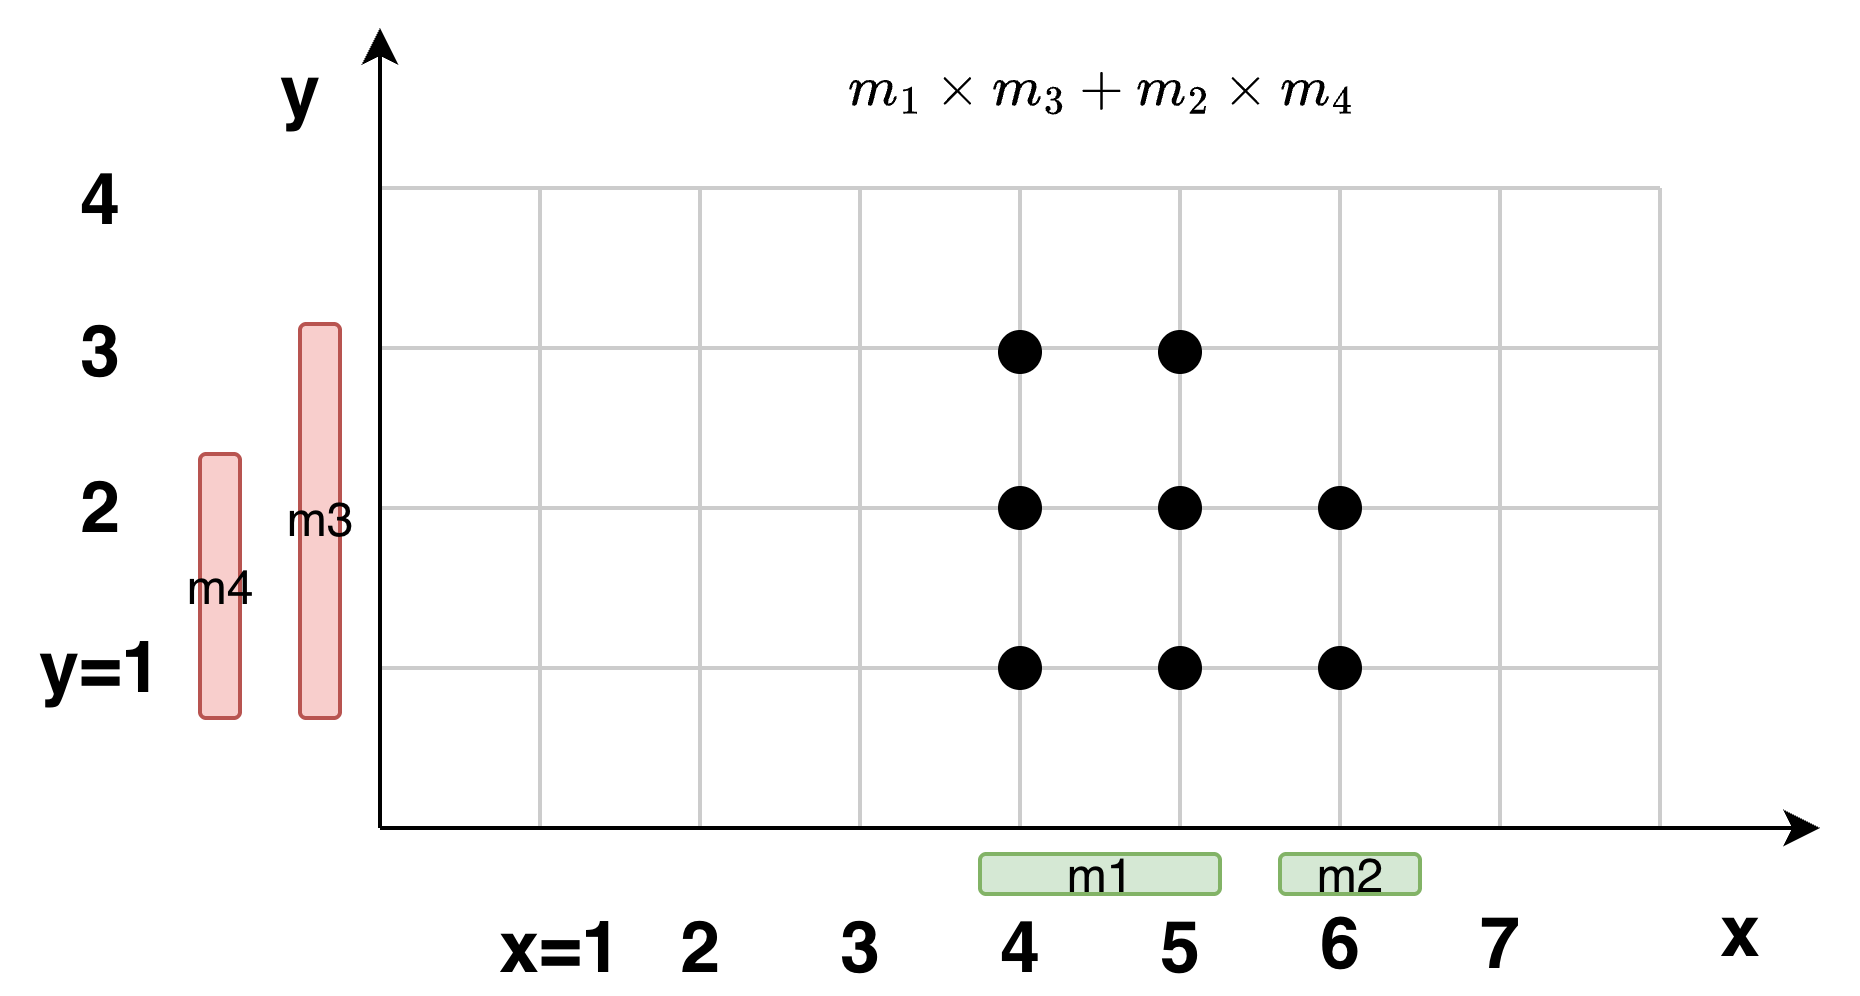
\includegraphics[width=0.8\textwidth]{figures/Ex1.drawio.png}
\end{figure}

\textbf{Example:} We show that how to use smaller resource to construct a larger resource; the atomic resource can be a ``line'' (e.g. $m_1$). Note that the ``shape'' does not need to be connected.

\textbf{Question:} How to define the partial order relation $\leq$?

\end{frame}

\begin{frame}[fragile]
    \frametitle{Choice Algebra: Partial Order}

\textbf{Intuition:} The partial order relation $\leq$ is ``entailment'' relation in the logic, where $a \leq b$ means $\forall \phi. a \models \phi \impl b \models \phi$.

% \textbf{Problem:} We have both over- and under- modality, and under- modality is contravariant.

\textbf{Intuition:} Assume $a\leq a + b$ since the $a + b$ contains ``more choices''. A reachability holds with smaller resource (choices) then also holds with larger resource.

\begin{figure}
    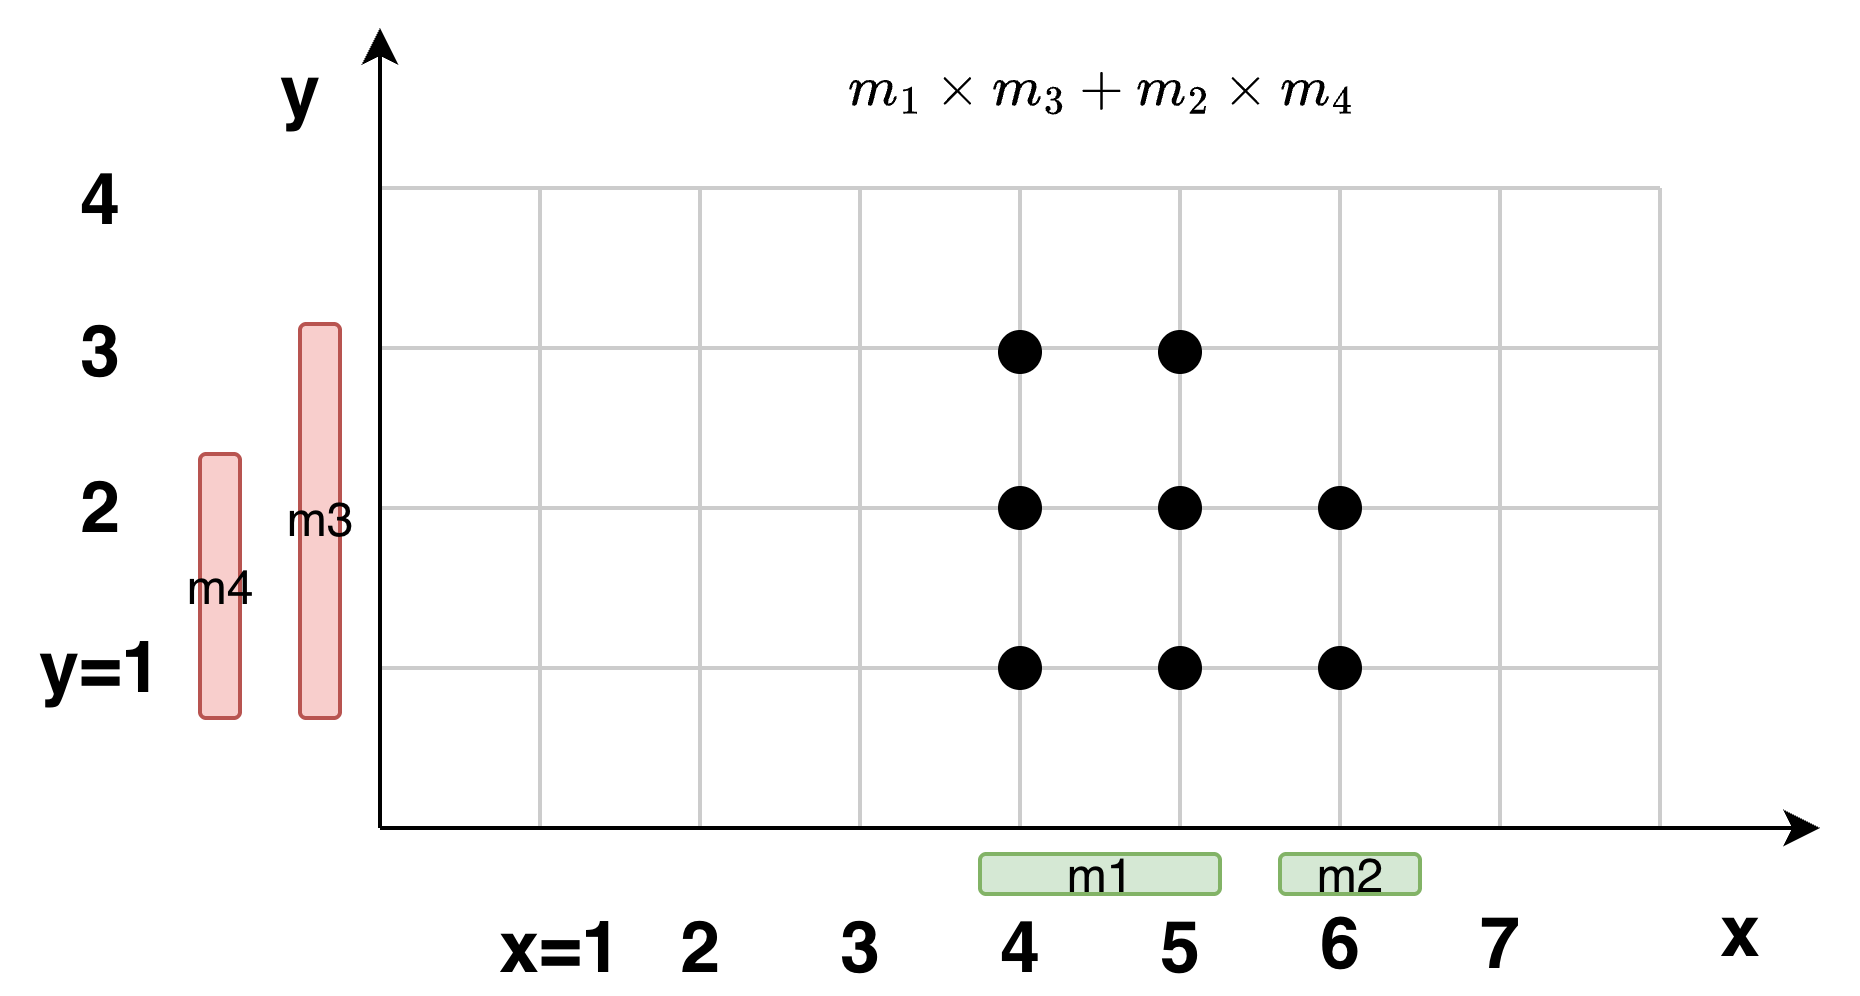
\includegraphics[width=0.8\textwidth]{figures/Ex1.drawio.png}
\end{figure}


\end{frame}

\begin{frame}[fragile]
    \frametitle{Choice Algebra: Partial Order}

\textbf{Question:} Compare $m_1$ with $m_1 \times m_2$?

\textbf{Intuition:} The $m_1 \times m_2$ can contains useless choices ($m_2$). 

\textbf{Observation:} If we have a set of choices $m_1 \times m_2$, we can projects thus choices into $\Dom{m_1}$ to recover $m_1$, the reverse is not true.

\textbf{Intuition:} $m_1 \leq m_1 \times m_2 + m_3$.

\begin{definition}[Partial Order]
    $m_1 \leq m_4$ iff $\exists m_2\;m_3. m_1 \times m_2 + m_3 = m_4$.
\end{definition}

\begin{lemma}[Bifunctoriality]
    $m_1 \leq m_2 \land m_3 \leq m_4 \impl m_1 \times m_3 \leq m_2 \times m_4$.
\end{lemma}

\end{frame}

\begin{frame}[fragile]
    \frametitle{Choice Logic}

\begin{definition}[Choice Logic] A choice logic is an intuitive logic with $*$, $\wand$, and $\oplus$ operators.
\end{definition}
\begin{itemize}
    \item $m \models \phi * \psi$ iff $\exists m_1\; m_2. m_1 \times m_2 \leq m \text{ and } m_1 \models \phi \text{ and } m_2 \models \psi$.
    \item $m \models \phi \wand \psi$ iff $\forall m'. m' \models \phi  \impl m' \times m \models \psi$.
    \item $m \models \phi \oplus \psi$ iff $\exists m_1, m_2. m_1 + m_2 \leq m \text{ and } m_1 \models \phi \text{ and } m_2 \models \psi$.
    \item $m \models P$ iff $\exists \sigma \in m. \sigma(P)$.
    \item $m \models \true$ always; $m \models \false$ never.
    \item We write $\models \phi$ when $\textbf{1} \models \phi$ holds (note that $\textbf{0}$ cannot model any proposition).
\end{itemize}

\begin{definition}[Underapproximation Modality]
    \begin{itemize}
        \item $m \models \boxtimes_5 \phi$ iff $\{\sigma ~|~ \{\sigma\} \models \phi \land \Dom{\sigma} = \Code{FV}(\phi) \} \leq m$.
    \end{itemize}
\end{definition}

\begin{definition}[Entailment]
    $\phi \models \psi$ holds, if for all $m$, $m \models \phi$ implies $m \models \psi$.
\end{definition}

\end{frame}

\begin{frame}[fragile]
    \frametitle{Choice Logic: Monotonicity}

    \begin{lemma}[Merge rule]
        $m \models \boxtimes_5 P_1 \oplus \boxtimes_5 P_2$ iff $m \models \boxtimes_5 (P_1 \lor P_2)$.
    \end{lemma}


\begin{lemma}[Kripke's Monotonicity]
        $m \leq m'$ and $m \models \phi$ implies $m' \models \phi$.
\end{lemma}

\begin{lemma}[Overapproximation]
    $\models P \impl Q$ holds, and $m \models P$ then $m \models Q$.
\end{lemma}

\begin{lemma}[Underapproximation]
    $\models P \impl Q$ holds, and $m \models \boxtimes_5 Q$ then $m \models \boxtimes_5 P$.
\end{lemma}

\end{frame}

\begin{frame}[fragile]
    \frametitle{Choice Logic: Examples}

    \begin{figure}
        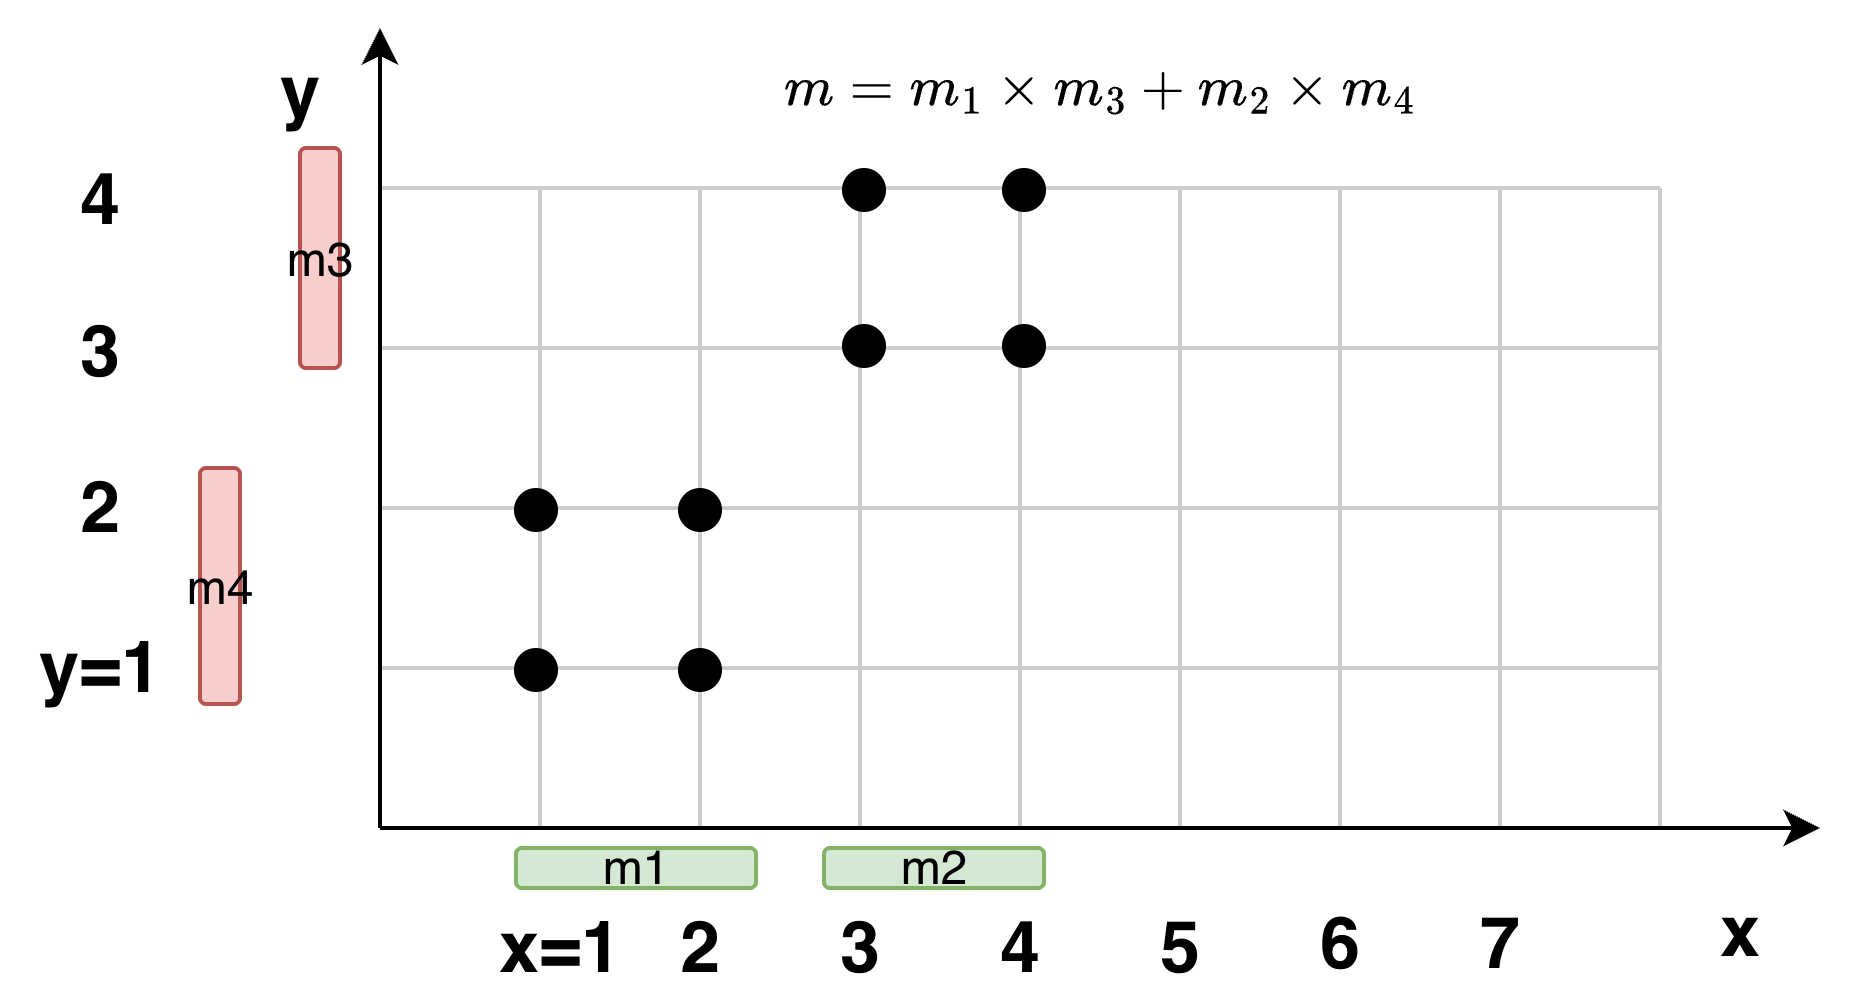
\includegraphics[width=0.8\textwidth]{figures/Ex2.drawio.png}
    \end{figure}

\textbf{Example:} We show that $m \models \boxtimes_5 (1 \leq x \leq 4)$.
\begin{itemize}
    \item $m_1 \times m_3 \leq m_1 \models \boxtimes_5 (1 \leq x \leq 2)$ by definition of $\boxtimes_5$.
    \item $m_2 \times m_4 \leq m_2 \models \boxtimes_5 (3 \leq x \leq 4)$ by definition of $\boxtimes_5$.
    \item $m \models \boxtimes_5 (1 \leq x \leq 2) \oplus \boxtimes_5 (3 \leq x \leq 4)$ by definition of $\oplus$.
    \item $m \models \boxtimes_5 (1 \leq x \leq 4)$ by merge rule. 
\end{itemize}
\end{frame}

\begin{frame}[fragile]
    \frametitle{Choice Logic: Examples}

    \begin{figure}
        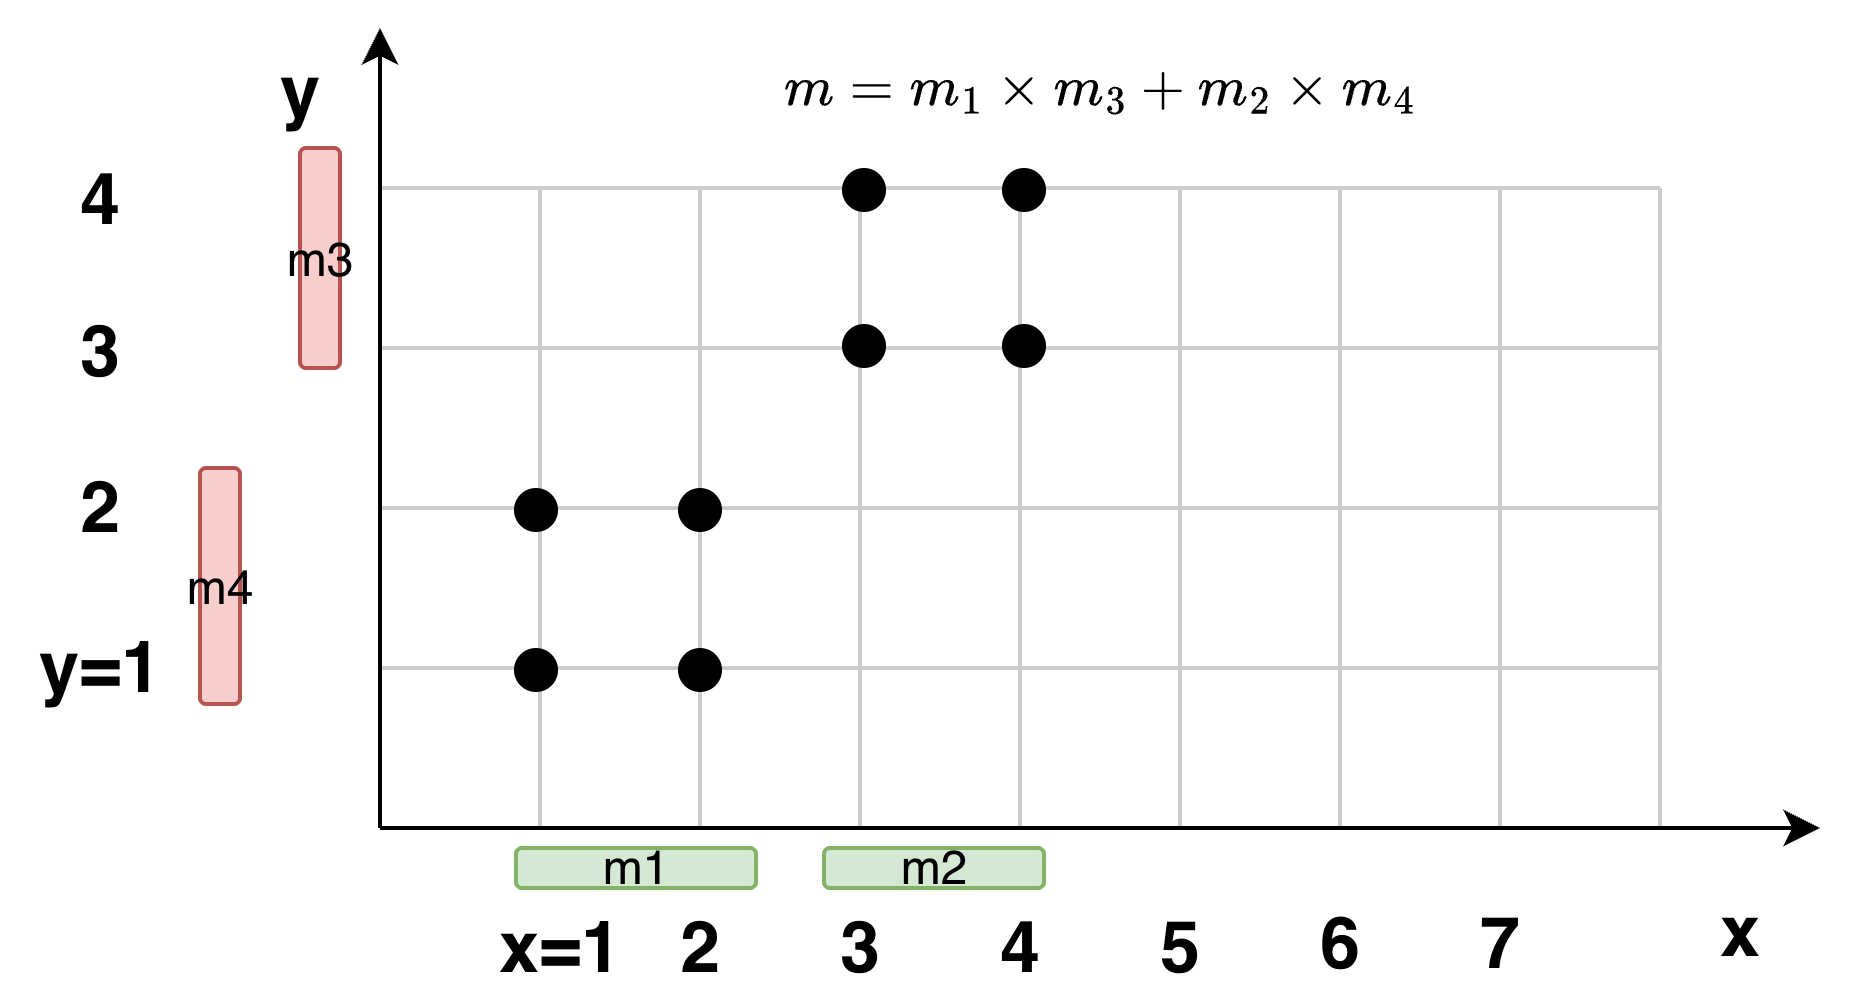
\includegraphics[width=0.6\textwidth]{figures/Ex2.drawio.png}
    \end{figure}

\textbf{Intuition:} If we don't have $\oplus$ operator, we cannot prove it!
\begin{itemize}
    \item Notice that $m$ which has domain $\{x,y\}$ however the property has domain $\{x\}$. Thus we need docompose $m$ into a form $m_x \times m_y$ (a rectangle).
    \item However, we cannot find a rectangle $\leq m$ and still can cover $1 \leq x \leq 4$. 
    \item The $+$ allows us to use the ``reminder'' after decomposition.
\end{itemize}
\end{frame}

\begin{frame}[fragile]
    \frametitle{Choice Logic: compare with previous version}

\begin{figure}
    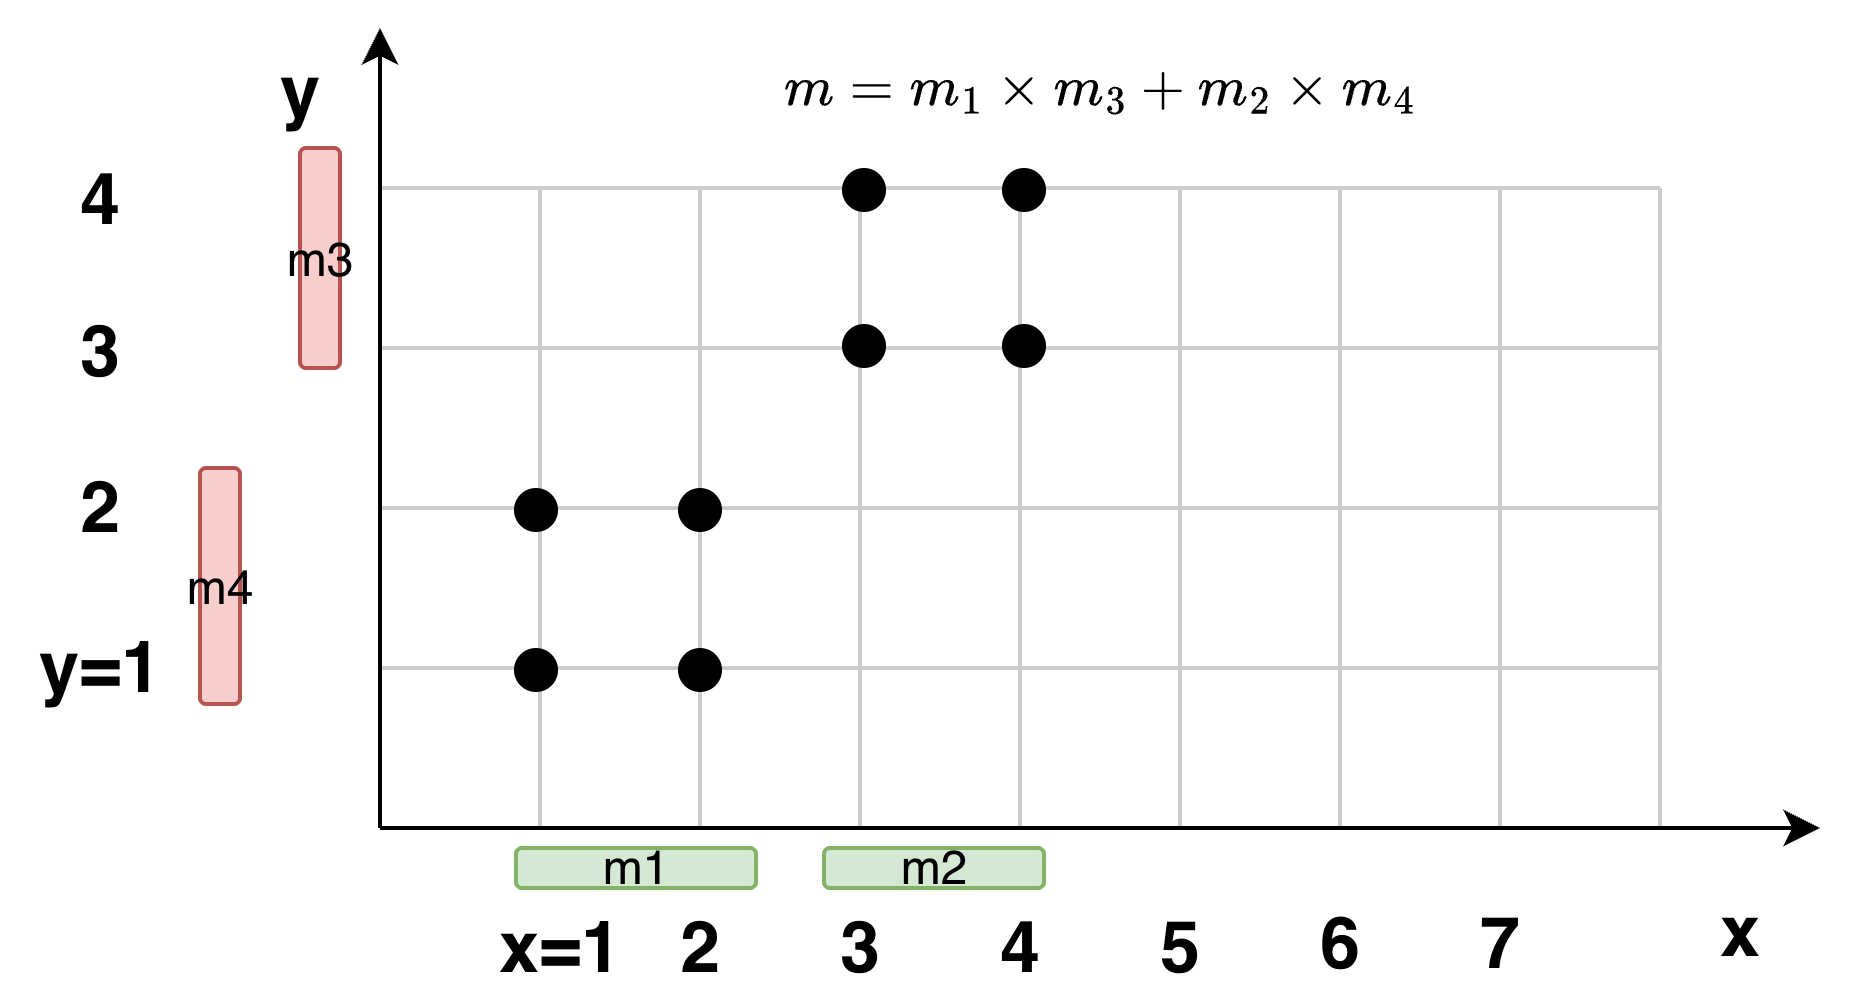
\includegraphics[width=0.6\textwidth]{figures/Ex2.drawio.png}
\end{figure}

\textbf{Version 1: model} We build a whole model to record the relation of choices, i.e., we record $m$, $m_1$, $m_2$, $m_3$, $m_4$, $m_1 + m_2$, $m_3 + m_4$, and their relations.
\begin{itemize}
    \item Each time we talk about $m_3$, we still remember $m$.
    \item Thus we know $m_3 \times m_2$ is valid (since $m_3 \times m_2 \leq m$).
    \item We also know $(m_1 + m_2) \times (m_3 + m_4)$ is invalid.
    \item We also don't have $+$ operator, since the model contains all valid sums.
\end{itemize}
\end{frame}

\begin{frame}[fragile]
    \frametitle{Choice Logic: compare with previous version}

\begin{figure}
    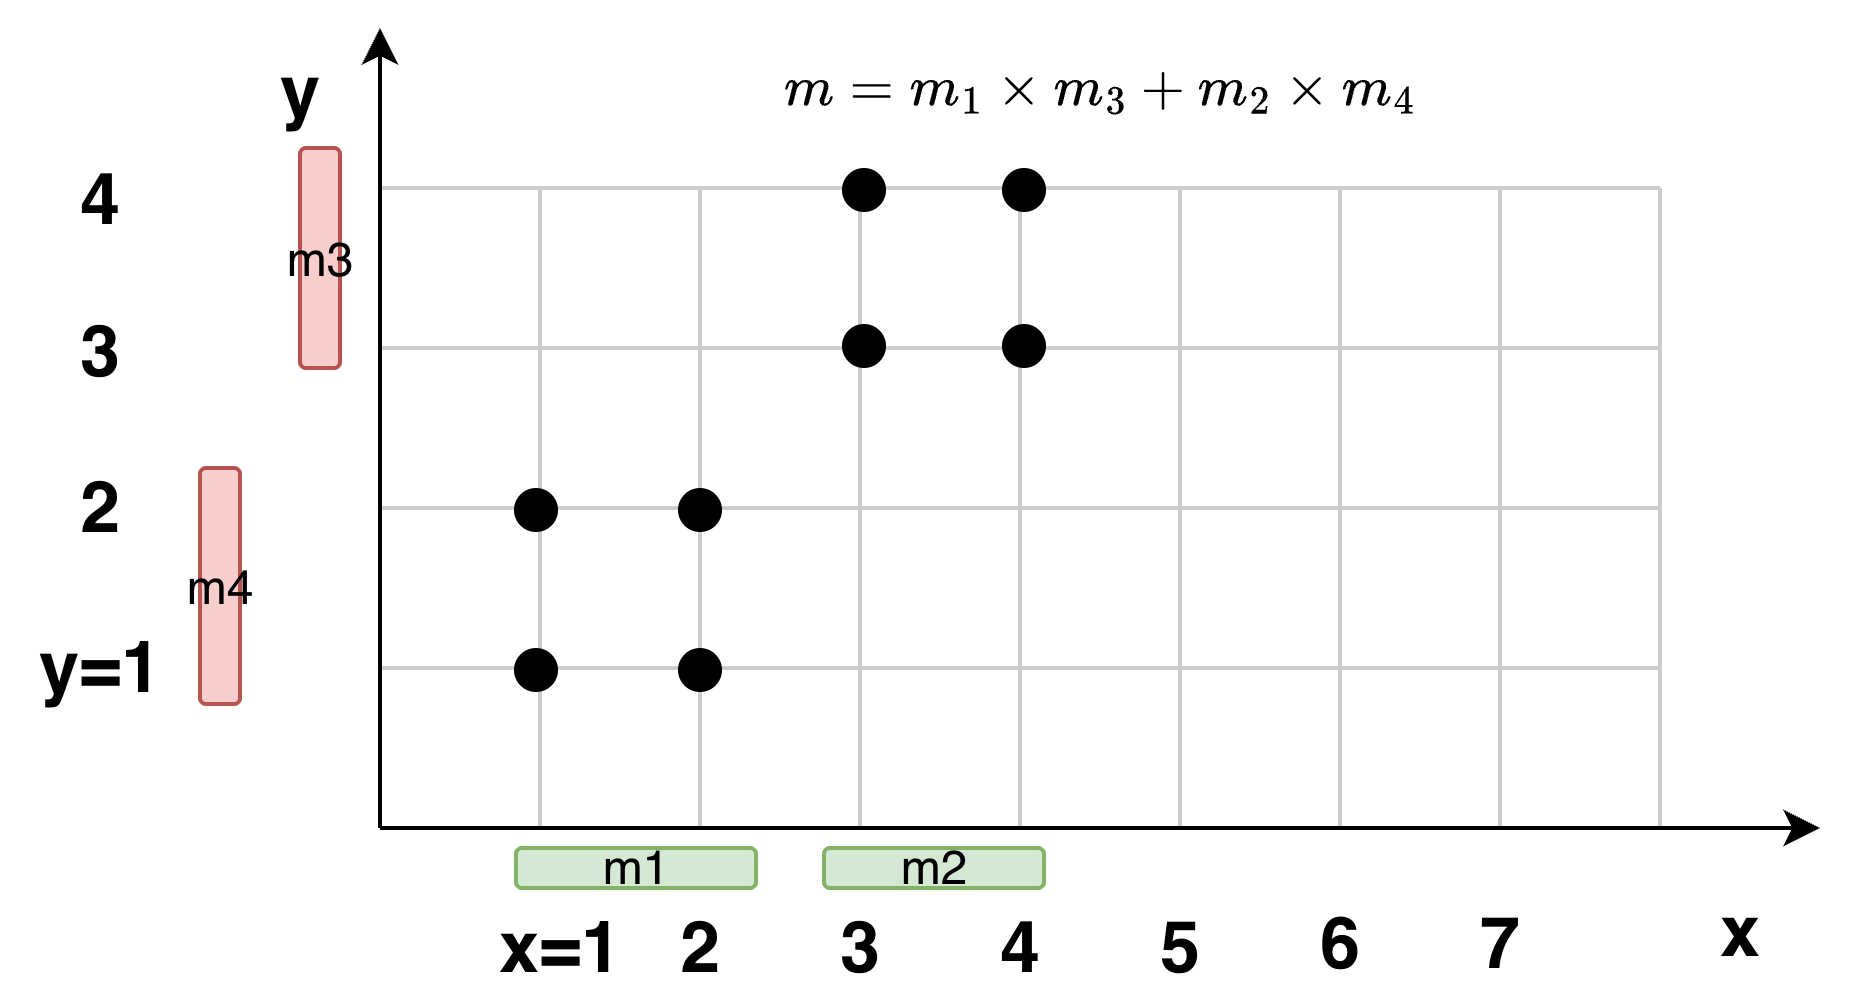
\includegraphics[width=0.6\textwidth]{figures/Ex2.drawio.png}
\end{figure}

\textbf{Version 1: $(\Sigma^+, \Sigma^-)$} We build a whole model to record the relation of choices, i.e., we record $m$, $m_1$, $m_2$, $m_3$, $m_4$, $m_1 + m_2$, $m_3 + m_4$, and their relations.
\begin{itemize}
    \item Each time we talk about $m_3$, we still remember $m$.
    \item Thus we know $m_3 \times m_2$ is valid (since $m_3 \times m_2 \leq m$).
    \item We also know $(m_1 + m_2) \times (m_3 + m_4)$ is invalid.
    \item We also don't have $+$ operator, since the model contains all valid sums.
\end{itemize}
\end{frame}

\begin{frame}[fragile]
    \frametitle{Choice Logic: compare with previous version}

\begin{figure}
    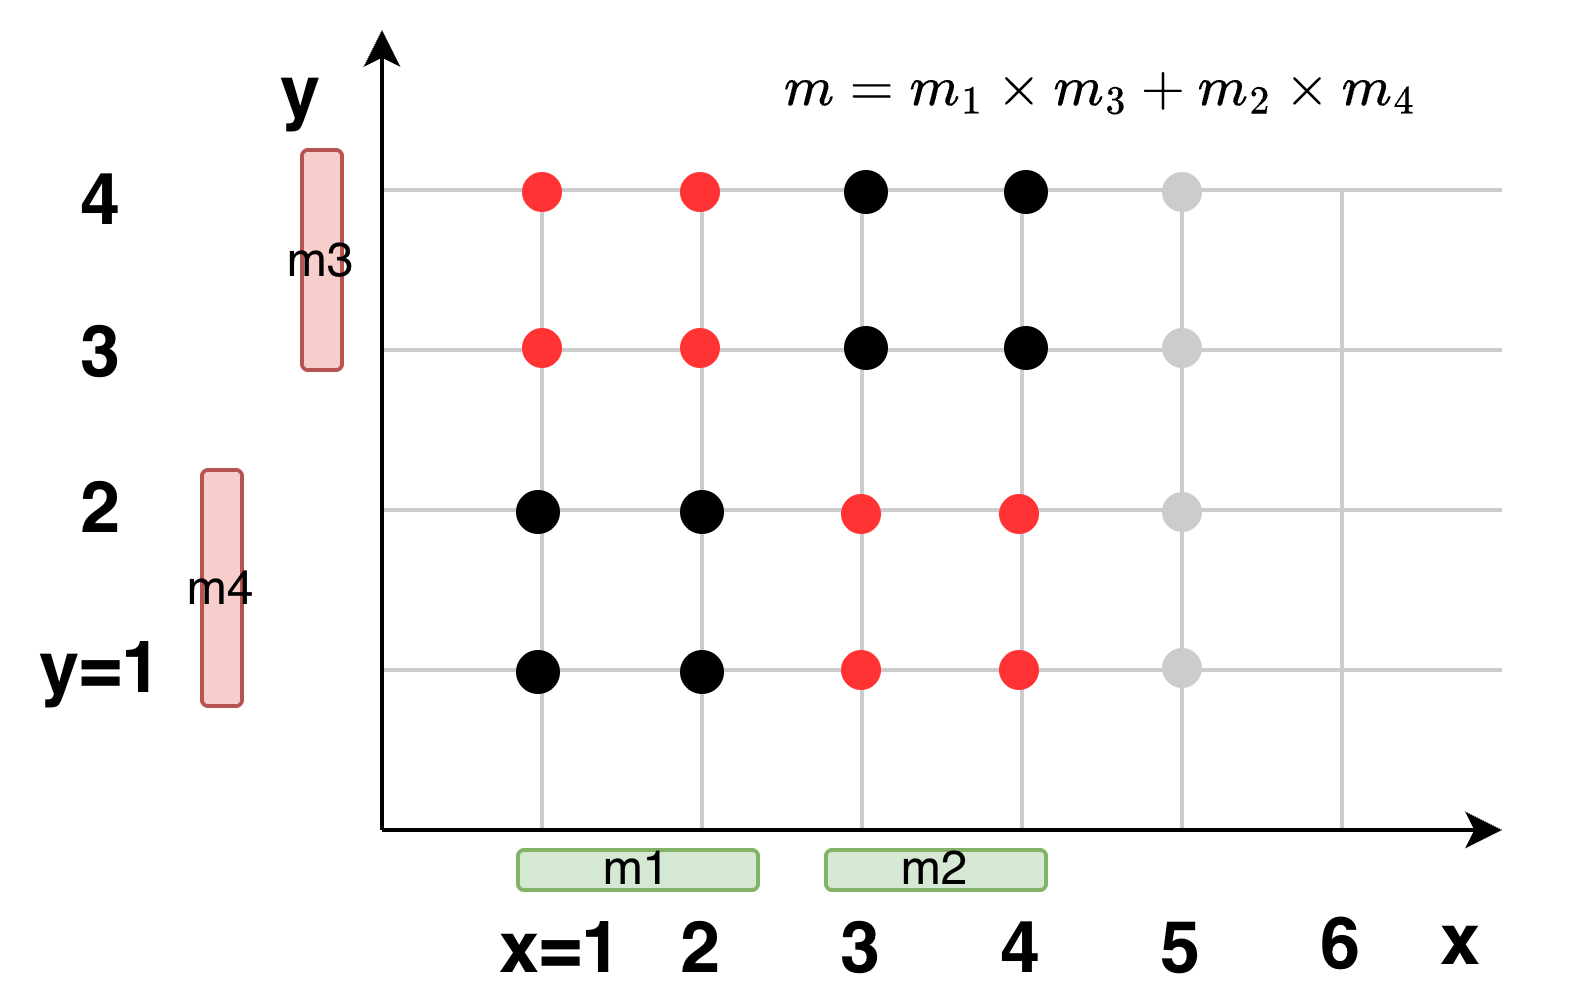
\includegraphics[width=0.6\textwidth]{figures/Ex3.drawio.png}
\end{figure}

\textbf{Version 2: $(\Sigma^+, \Sigma^-)$} we express $m$ as a set positive set (black points) and negative set (red points).
\begin{itemize}
    \item The red nodes are ``disallowed choices'', thus we can always track them -- even in $m_3$ that has a different domain.
    \item $m_1 \times m_3$ is empty since all choices are cancelled out by the red nodes.
    \item Gray points are nagtive but can be ignored, since they are never used.
\end{itemize}
\end{frame}

\begin{frame}[fragile]
    \frametitle{Choice Logic: compare with previous version}

\textbf{Problem:} All complex definition in previous version come from we want to use single resource to track knowledge even out of its domain.

\textbf{Intuition:} We don't want to lose information (e.g., negative choices), however we don't know where to store them since $\leq$ relation always drop information.

\textbf{Idea:} We introduce $m = m_1 \times m_2 + m_3$, where $m_1 \times m_2 \leq m$ indeed lose the information $m_3$, but the $+$ allows us to reuse this reminder.

\mprooftr{50mm}{
 $m_1 \times m_2 \models \boxtimes_5 \phi_1$ \quad $m_3 \models \boxtimes_5 \phi_2$
}{Merge rule}{
 $m_1 \times m_2 + m_3 \models \boxtimes_5 (\phi_1 \lor \phi_2)$}

\end{frame}

\begin{frame}[fragile]
    \frametitle{Choice Logic: Persistency}

\textbf{Idea:} Persistent proposition $\phi$ means $\phi$ holds without exclusive ownership; persistent proposition can be duplicated: $\phi * \phi \iff \phi$.

\textbf{Intuition:} We know that pure proposition $P$ is persistent, and singleton coverage is also persistent.

\textbf{Problem:} $\boxtimes_5 (x = 1) * \boxtimes_5 (x = 1)$ is not well-formed.

\begin{definition}[Addition and Multiplication] There are partial operations:
    \begin{itemize}
        \item $m_1 + m_2 \doteq m_1 \cup m_2$ when $\Dom{m_1} = \Dom{m_2}$.
        \item $m_1 \times m_2 \doteq \{ \sigma_1 \cup \sigma_2 ~|~ \sigma_1 \in m_1 \land \sigma_2 \in m_2 \}$
        \item when $\forall \sigma_1 \in m_1, \forall \sigma_2 \in m_2. \forall x. x \in \Dom{\sigma_1} \land x \in \Dom{\sigma_2} \implies \sigma_1(x) = \sigma_2(x)$.
    \end{itemize}
\end{definition}

\begin{lemma}[Idempotency] $|m| \leq 2$ implies $m \times m = m$.
\end{lemma}

\end{frame}

\begin{frame}[fragile]
    \frametitle{Choice Logic: Persistency}

\begin{definition}[Persistency]
    \begin{itemize}
        \item $m \models \Box \phi$ iff there exists a singleton resource $m'$ (i.e., $|m'| = 1$) such that $m' \leq m$ and $m' \models \phi$.
    \end{itemize}
\end{definition}

\textbf{Intuition:} We ensure that there is no choice to be made.

\textbf{Note:} The resource $\textbf{0}$ cannot model any proposition; thus, we do not consider it.

\begin{lemma}[Persistence Elimination] $m \models \Box \phi$ implies $m \models \phi$.
\end{lemma}

\begin{lemma}[Persistence Duplicatable] $m \models \Box \phi$ implies $m \models \Box \phi * \Box \phi$.
\end{lemma}

\end{frame}

\begin{frame}[fragile]
    \frametitle{Choice Logic: Persistency}

\begin{lemma}[Persistence Pure] A pure proposition $P$ is persistent: $P \models \Box P$.
\end{lemma}
\begin{proof} A valid pure proposition holds under $\textbf{1}$. 
\end{proof}

\begin{lemma}[Persistence Idempotency] $\Box \phi \models \Box \Box \phi$.
\end{lemma}

\begin{lemma}[Persistence Conjunction] $\Box \phi_1 \land \phi_2 \models \Box \phi_1 * \phi_2$.
\end{lemma}
\begin{proof} Note that if a singleton resource $m' \leq m$, then we actually have $m' \times m = m$. This rule is not a part of standard $!$ modality in linear logic.
\end{proof}

\end{frame}


\begin{frame}[fragile]
    \frametitle{Choice Logic: Other modalities}

\begin{definition}[Modality]
    \begin{itemize}
        \item $m \models \diamond_5 \phi$ iff $\exists \sigma \in m. \{\sigma\} \models \phi$.
        \item \textbf{Note:} the persistency modality $\Box$ is exactly the possibility modality $\diamond_5$ in S5.
        \item $m \models \Box_5 \phi$ iff $\forall \sigma \in m. \{\sigma\} \models \phi$.
        \item Break the Kripke's Monotonicity: More resource doesn't mean still correct.
    \end{itemize}
\end{definition}

\textbf{Note:} The $\diamond_5$ modality works like ``overapproximation'' and $\boxtimes_5$ modality works like ``underapproximation''.

\textbf{Example:} Consider type context $x{:}\ort{\Int}{\vnu > 0}, y{:}\urt{\Int}{\vnu > 0}: \vdash ...$
\begin{itemize}
    \item can be expressed as $\diamond_5 (x > 0) \land \boxtimes_5 (y > 0) \models ...$.
    \item can also be expressed as $\diamond_5 (x > 0) * \boxtimes_5 (y > 0) \models ...$ (persistence conjunction rule)
    \item Overapproximation is presistency.
\end{itemize}
\end{frame}

\end{document}
